\documentclass{article}\usepackage[]{graphicx}\usepackage[]{color}
% maxwidth is the original width if it is less than linewidth
% otherwise use linewidth (to make sure the graphics do not exceed the margin)
\makeatletter
\def\maxwidth{ %
  \ifdim\Gin@nat@width>\linewidth
    \linewidth
  \else
    \Gin@nat@width
  \fi
}
\makeatother

\definecolor{fgcolor}{rgb}{0.345, 0.345, 0.345}
\newcommand{\hlnum}[1]{\textcolor[rgb]{0.686,0.059,0.569}{#1}}%
\newcommand{\hlstr}[1]{\textcolor[rgb]{0.192,0.494,0.8}{#1}}%
\newcommand{\hlcom}[1]{\textcolor[rgb]{0.678,0.584,0.686}{\textit{#1}}}%
\newcommand{\hlopt}[1]{\textcolor[rgb]{0,0,0}{#1}}%
\newcommand{\hlstd}[1]{\textcolor[rgb]{0.345,0.345,0.345}{#1}}%
\newcommand{\hlkwa}[1]{\textcolor[rgb]{0.161,0.373,0.58}{\textbf{#1}}}%
\newcommand{\hlkwb}[1]{\textcolor[rgb]{0.69,0.353,0.396}{#1}}%
\newcommand{\hlkwc}[1]{\textcolor[rgb]{0.333,0.667,0.333}{#1}}%
\newcommand{\hlkwd}[1]{\textcolor[rgb]{0.737,0.353,0.396}{\textbf{#1}}}%
\let\hlipl\hlkwb

\usepackage{framed}
\makeatletter
\newenvironment{kframe}{%
 \def\at@end@of@kframe{}%
 \ifinner\ifhmode%
  \def\at@end@of@kframe{\end{minipage}}%
  \begin{minipage}{\columnwidth}%
 \fi\fi%
 \def\FrameCommand##1{\hskip\@totalleftmargin \hskip-\fboxsep
 \colorbox{shadecolor}{##1}\hskip-\fboxsep
     % There is no \\@totalrightmargin, so:
     \hskip-\linewidth \hskip-\@totalleftmargin \hskip\columnwidth}%
 \MakeFramed {\advance\hsize-\width
   \@totalleftmargin\z@ \linewidth\hsize
   \@setminipage}}%
 {\par\unskip\endMakeFramed%
 \at@end@of@kframe}
\makeatother

\definecolor{shadecolor}{rgb}{.97, .97, .97}
\definecolor{messagecolor}{rgb}{0, 0, 0}
\definecolor{warningcolor}{rgb}{1, 0, 1}
\definecolor{errorcolor}{rgb}{1, 0, 0}
\newenvironment{knitrout}{}{} % an empty environment to be redefined in TeX

\usepackage{alltt}
\usepackage{Sweave}
\usepackage{float}
\usepackage{graphicx}
\usepackage{hyperref}
\usepackage[svgnames]{xcolor}
\usepackage[T1]{fontenc}
\hypersetup{
    colorlinks=true,
    linkcolor=blue,
    filecolor=magenta,      
    urlcolor=cyan,
}

\urlstyle{same}
\usepackage{tabularx}
\usepackage{siunitx}
\usepackage{amssymb} % for math symbols
\usepackage{amsmath} % for aligning equations
\usepackage{textcomp}
\usepackage{mdframed}
\usepackage{natbib}
%\bibliographystyle{..//references/styles/besjournals.bst}
\usepackage[small]{caption}
\setlength{\captionmargin}{30pt}
\setlength{\abovecaptionskip}{0pt}
\setlength{\belowcaptionskip}{10pt}
\topmargin -1.5cm        
\oddsidemargin -0.04cm   
\evensidemargin -0.04cm
\textwidth 16.59cm
\textheight 21.94cm 
%\pagestyle{empty} %comment if want page numbers
\parskip 7.2pt
\renewcommand{\baselinestretch}{1.5}
\renewcommand{\rmdefault}{qag} % Arial
\renewcommand{\sfdefault}{qag} % Arial
\parindent 0pt
%\usepackage{lineno}
%\linenumbers

\newmdenv[
  topline=true,
  bottomline=true,
  skipabove=\topsep,
  skipbelow=\topsep
]{siderules}
\IfFileExists{upquote.sty}{\usepackage{upquote}}{}
\begin{document}

\noindent {\LARGE{\textbf{Landowner Document: OUTLINE}}}
\vspace{3ex}\\
{\Large{\textbf{Family Forest Carbon Program}}}
  \begin{itemize}
  
  \item What you do on your land is important.  The Family Forest Carbon Program is a program that is focused on payments to landowners for management choices that increase the amount of carbon stored on their land. You may already have read other documents from similar programs (UMass/UVT carbon document, UVT resilience document, MA DCR carbon document that gets sent to everyone with their management plans, etc.) You may also have heard about programs from the Natural Resource Conservation Service or Foresters for the Birds. These programs have a lot of similarities---all of them ask you to first think about why you own and love your land, and then to work with a professional to choose from a list of options for managing your land well, with a long-term plan in mind. You may also decide that the right fit for you is to have your land managed by nature---not by people---as forest reserve. We'll walk you through some of the details of the Family Forest Carbon Program and help you decide whether this is the right fit for you.
  
  \item Your land not only impacts you and your community but also the plants and wildlife that call your land home. The decisions you make about your land can also greatly impact the climate. Forests are one of the few natural and essential tools we have to draw down carbon from the atmosphere and turn it into wood, roots and soil.
  \item  The most important thing you can do to help fight climate change is to ensure that your land remains a forest now and to decide what will happen to your forest in the future.
  \item That is why the decisions you make about managing your land can be a major positive influence on our environment and benefit forest income, wildlife, provide clean water, establish a resilient ecosystem and mitigate climate change.   
  \end{itemize}

  \begin{itemize}
  \item Your forest may be small but landowners like you own 80\% (USDA NRCS, 2011) of New England and New York forests. The small forest size has often made it challenging to access incentive programs that can help you to do carbon-beneficial forest management on your land.
  
  \item The Family Forest Carbon Program, which is a collaboration between the American Forest Foundation and the Nature Conservancy, works with you to mitigate climate change and maintain resilient forests. 

  {\begin{figure} [H]
  -\begin{center}
  -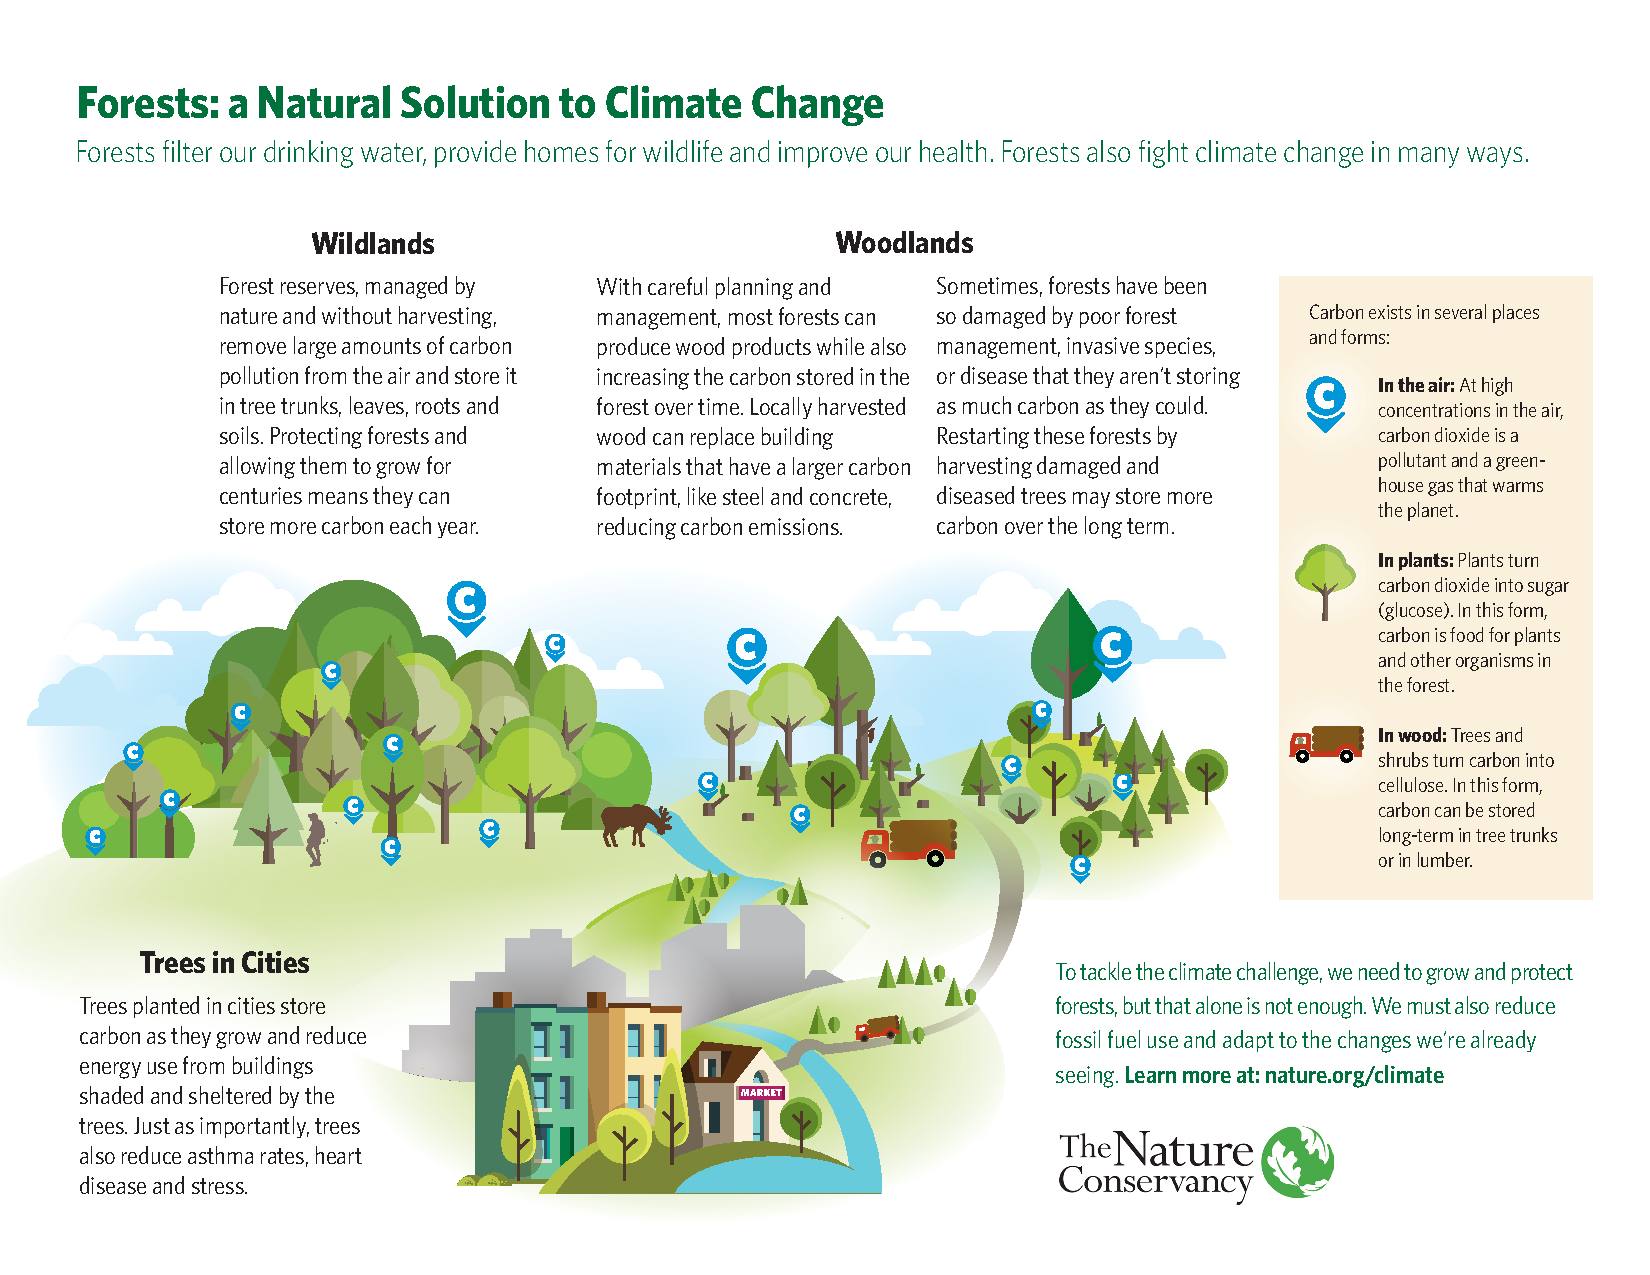
\includegraphics[width=16cm]{..//figures/TNC-forestC.pdf}\label{fig:carbon}
  -\end{center}
  -\end{figure}}

  %\item Across the United States, 38\% of forests are owned by families or individuals. The majority of forest landowners have 20 to 500 acres but these families are unable to contribute to carbon markets due to high costs and inaccessibility.  By implementing the Family Forest Carbon Program into New England, we can help resolve some of these complexities by increasing our carbon sequestration potential by opening XXX million acres of forestland. 
  
   
  \end{itemize}

{\Large{\textbf{Is the Family Forest Carbon Program a good fit for you?}}} \\
\vspace{2ex}\\
{\large{\textbf{Benefits include:}}}
  \begin{itemize}
  \item Payments to help cover the cost of managing your land: sources include public dollars to grow more carbon and improve other forest values, private foundations with an interest in forests, or carbon credits traded in carbon markets.
  \item Guidance from a forester: A trained professional forester will work with you to consider your values for your land and write a long-term management plan that considers clean water, wildlife habitat, and production of wood products while increasing the amount of carbon stored on your land over 20 years.
  \item Return on Investment: investment in forest management on your land doesn't just help you and the local wildlife but it amplifies the economy through the creation of jobs for foresters and loggers and supports other sectors such as tourism, outdoor recreation and agriculture. 
  \end{itemize}

{\Large{\textbf{The Family Forest Carbon Practices}}}
  \begin{itemize}
  \item This program began in response to the early- and mid-stage carbon markets, which were generally ineffective for family forest landowners in New England due to large parcel size requirements. The Family Forest Carbon Program helps family forest landowners design and implement a 20-year forest management plan that focuses on carbon sequestration---primarily on the carbon stored in trees, or the aboveground carbon stock. 
  \item Simultaneously, we aim to take a practice-based approach to best suit \textit{your} needs and to manage your forest the way you want it to be managed. It is crucial that you don't lose sight of the reasons you own and enjoy your woods: whether it is a place to enjoy nature, a home for wildlife, a family legacy you wish to protect, a financial investment, a source of heat or maple syrup or furniture or lumber from the wood you harvest. Your management decisions should reflect all of your values---managing simply for a short-term increase in carbon stock makes as little sense as managing just for a short-term economic gain.
  \item The Family Forest Carbon Program includes 9 possible practices, which are considered ``good for the climate'' and were first established in 2019 by a team from the Nature Conservancy, American Forest Foundation and the US Forest Service. With help from a group of more than 20 stakeholders---including County/Service foresters and state agency staff, landowners, scientists, private foresters, loggers, land trusts, and others---we narrowed these existing resources down to the nine practices listed below. 
  \item These practices increase carbon stock and benefit the land on which they are applied within 20 years (the timeframe of the Family Forest Carbon Program contracts). Most of these practices show carbon benefits immediately. A few, such as reforestation, take several years to begin showing carbon benefits.
  \item All of the practices on this list are long-term commitments that positively affect the environment and enhance habitats for wildlife. We did not rank these practices and we have no intention to dictate which practice is the ``best'' option for you, and we certainly don't want to determine which is the ``best'' one for your neighbor! This a personal decision for you to make with your forester, thinking about all the values of your forest and what will leave you feeling good about and the impact you have made. In an ideal world, we'd like to see different landowners choose different practices but all practices are deemed essential and a crucial step towards positive change.
  \item All forests are different and the conditions of your forest will likely best match one or two of these practices. Your forester will help you make that determination. It's not entirely up to you what is best for your forest and the environment, but by openly and clearly communicating with your forester, you can chose the best practice to match your needs and values. 
  
  \begin{centering}   
\fbox{ {\setlength{\fboxrule}{2pt}
\begin{minipage}{6.5 in}
{\large{\textbf{\textcolor{DarkGreen}{FOREST RESILIENCE:}}}}\\
  Forest Resilience is ``the capacity of a forest to respond to a disturbance by resisting damage or stress and recovering quickly'' (Catanzaro \textit{et al.}, 2016).
  
  Our forests are vulnerable to land conversion, invasive plants, insects, and diseases, heavy deer and moose browsing and climate change. Your forest provides clean water, wildlife habitats, recreational opportunities and forest products while also sequestering carbon from the atmostphere. By keeping your forest a forest, it will continue to be resilient and help reduce the risks of climate change. Though the Family Forest Carbon Program uses carbon as a way to measure its success, all nine practices work to build resilience to stressors.
  \end{minipage}}}
\end{centering}
  
  \item By joining the Family Forest Carbon Program, you will become part of a team which includes: 
    \begin{enumerate}
    \item A Forester: who will help you write a management plan that fits your values and makes sense for your landscape, as well as record the types of trees and amount of carbon on your land to begin with. Some of the practices also require help from a logger/harvester, who will cut and remove trees and turn them into wood products.
    \item The Family Forest Carbon Program Team: led by American Forest Foundation, you will work with staff to sign up, get an initial payment, and have program staff visit your land over the coming years to monitor the growth of your forest and carbon stored within it
    \item And most importantly you! You must share what is most important to you with your forester so that the forester and harvester can help you maintain what you value about your forest. 
    \end{enumerate}

  \item You and your team will then develop a forest management plan that follows one of the nine possible practices: (please note the first three practices are not eligible for FFCP payments)
  \item NOTE: we need a few sentence narrative descriptions of each individual practice (Cat has added some contet, Todd and Laura to help edit)

    \begin{enumerate}
    \item Avoid forest loss: Reduce or eliminate conversion of forest to non-forest use since forest lands contain more carbon than most other land uses.
    %\item Avoiding pre-salvage logging: Leaving dead or dying trees and allowing natural mortality and decomposition from disturbances. For example, leaving hemlock or ash to add carbon to soil and downed wood carbon pools. Also, avoiding salvage logging following severe natural disturbances, (e.g. hurricanes, tornadoes, ice storms). 
    \item Extending cutting cycles: Expanding from one 10-year management plan to two consecutive plans to allow for 10 years of additional growth before harvest.
    \item Planting trees along streets and in yards: Tree planting in urban and residential areas to increase overall sequestration and storage from enhancing the tree canopy. 
    \item Reforestation: Through seeding, stocking or passive reforestation, create a forest with a diversity of trees that reduce the risk of climate change.
    \item Creating regeneration with complexity: When forests are undergoing harvests, retention of a minimum number of large-diameter live trees, snags (see NEFF's Exemplary Forestry standards), and live-but-dying trees (future snags), enhancement of coarse woody debris, and limiting gap creation to 15\% to no more than 20\% of the parcel.
    \item Retaining more carbon in thinnings: Increased retention of live trees and slash during thinning practices, resulting in greater post-harvest stocking. Retain trees of a diversity of species.
    \item Establishing reserves: No harvesting over a 20-year period with intent to continue beyond 20 years (with exceptions for invasive removals or novel outbreaks of forest pests and pathogens). Preference given to sites with high carbon density (may include: soil organic carbon threshold; old growth characteristics---such as all-aged conditions, abundant CWD, large diameter trees) and low vulnerability sites with high species diversity or species composition with high proportion of future-adapted species. Reserves can cover an entire parcel, or can occur on part of a parcel. 
    \item Protecting regeneration from deer and moose: Actions to reduce over-browsing and protect regeneration from animal damage. Practices may include use of tree shelters, exclusion fencing, bud capping, or repellent sprays to reduce herbivore damage to desirable regeneration or planted stock. 
    \item Removing competing vegetation: Removal of heavy infestations of invasives that compete with regeneration, either pre- or post-harvest, or both. May include treatments designed to prevent the establishment of invasives (e.g. herbiciding).
    \end{enumerate}

  \item NOTE HERE: CAT NEEDS HELP WITH THIS INFORMATION
  \begin{itemize}
    \item Most of these practices require a 20 year contract and some require more than one year of activity on the land. Discussion of time commitment required for the program (in most cases, 20 year contract; for some practices, it will require more than one year’s worth of activity on the land, for example invasive treatments almost always have to be repeated)
    \item By the time of any payments, landowners must have a forest management or forest stewardship plan (do not need one at program entry)
    \item In all practices, you must maintain healthy soils.
    \item Risk (payments aren't guaranteed especially for practices with performance standards)
  \end{itemize}
  \end{itemize}
  
{\Large{\textbf{Eligible families and individuals}}}\\
\begin{itemize}
\item Eligible landowners must meet the following criteria:
  \begin{enumerate}
  \item Your land is within the eligible project areas (see map below)
  \item Your land is between 30 and 2,400 acres of non-industrial private forestland
  \item It must by legal for you to do your chosen practice on your land. For example, some landowners have conservation easements or are in protected areas like wetlands, that limit the types of land management they can legally do. As another example, if you are enrolled in a state "current use tax" program like Chapter 61 in Massachusetts or Use Value Appraisal in Vermont, you may be eligible for some of the practices but not others (NOTE FROM LAURA: Use this instead of already written - )
  \item You must be willing to sign a contract with the Family Forest Carbon Program, and plan to continue owning your land for the life of the contract (10 to 20 years, depending on the management practice you choose.)
  \end{enumerate}
\end{itemize}

{\begin{figure} [H]
  -\begin{center}
  -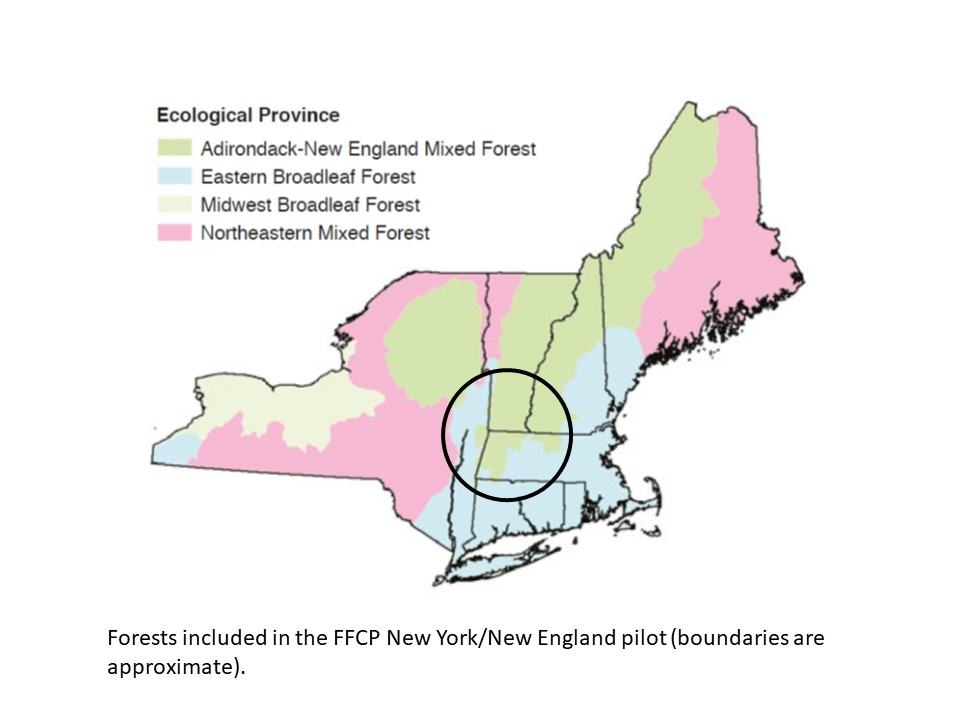
\includegraphics[width=14cm]{..//figures/map_for_ffcp.jpg}\label{fig:map}
  -\caption{This map is a rough estimate of eligible areas. Please contact the FFCP for the exact boundaries within your state.}
  -\end{center}
  -\end{figure}}
  
{\Large{\textbf{What about offsets?}}}
\begin{enumerate}
  \item offsets as a last resort
  \item but also as a needed policy tool
  \item offsets only look at carbon, but our practices look at much more than that
  \item not using offsets as an excuse -- need to take dramatic action to reduce emissions, and need to leave most of the carbon gains for drawdown
\end{enumerate}

%{\begin{figure} [H]
 % -\begin{center}
  %-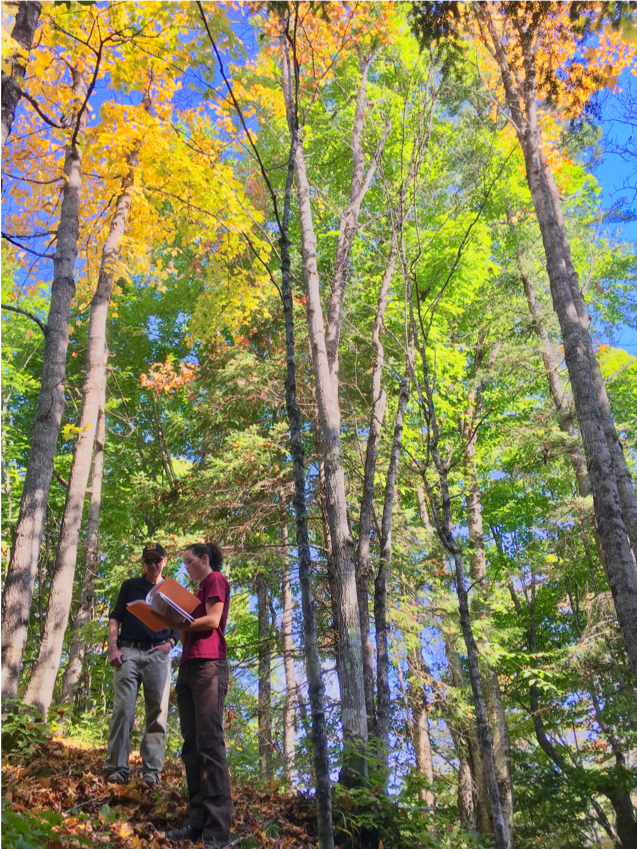
\includegraphics[width=8cm]{..//figures/forestimage.png}\label{fig:forest}
  %-\end{center}
  %-\end{figure}}


{\Large{\textbf{Why the Family Forest Carbon Program is so important now}}}

  \begin{itemize}
  \item Forests help fight the adverse effects of climate change by pulling carbon from the atmosphere and turning it into wood, roots and soil. The primary aim of the Family Forest Carbon Program will always be ``avoiding forest loss''. From a carbon standpoint, when a forest is converted to another land-use, a portion of the carbon stored in its trees is immediately lost as trees are cut, roots decay, and wood that isn't valuable enough to sell is often piled on site or used as mulch and other short-lived products. Every year after that, we lose carbon sequestration. Often called ``foregone sequestration'', this refers to the carbon that the forest used to pull from the atmosphere each year and turn into wood, roots, and soil.
  
  \item In New England, we lose 77 acres of forestland each day, which is over 28,000 acres in a year (Olofsson et al., 2016). The most important thing you can do as a family forest landowner is to keep your forest a forest so your trees can continue to sequester carbon and combat climate change.

  \item Wood is often not considered to be part of the carbon cycle, but it is. Once dried, wood is about 50\% carbon. If that wood is used in long-lived products like furniture and buildings, that carbon that was removed from the air while the tree was alive is stored almost indefinitely. In Massachusetts, the Fairbanks House is an extreme example---a timber frame house built circa 1641---of how wood can be a way to lock up and secure carbon for the long term. As states and countries and the world think about forests and climate change, they are trying to make sure that the wood we use is sustainably harvested (which yours will be), and that we don't take actions in places that have climate change policies in place (like New England) that reduce wood production here to the point that people start using less sustainable products that take more carbon to produce and ship.

  \item It is important that you pay particular attention to what wood products you generate and how these products can be used to store carbon in the long-term. None of these practices allow poor land management (``take the best and leave the rest''), large-scale clearcutting, or short-term decisions that reduce the ability of the forest to provide wood in the future. If you are choosing from our list of carbon-beneficial practices, the wood that comes out of those harvests is sustainable. Wood that is used to substitute for more carbon-intensive materials, like concrete, steel, heating oil or irresponsibly harvested wood from tropical forests has a huge carbon benefit. In this program specifically, we are not paying landowners for that carbon value, but that does not mean that it should be ignored as you think about how to manage your land.

  \item Many carbon-beneficial practices cost landowners money, at least in the near term. The Family Forest Carbon Program is paying for a change in behavior from the ``common practice'' or ``business as usual'' harvest to one that might leave more standing dead trees on site, to harvest less intensively or build fences to keep out deer, all of which cost the landowner money. Part of the money from a harvest will come from the Family Forest Carbon Program and then additional income will come from selling wood. Since wood is a form of forest carbon that has a value in the marketplace already, we don't include payments for it in the Family Forest Carbon Program.
  
  \item In most traditional carbon markets, carbon benefits are calculated by doing an exhaustive inventory on each piece of land, which is so costly that only those who own thousands of acres of land can afford to enroll in the markets. The Family Forest Carbon Program uses a different and more flexible approach, more like that used by existing state and federal programs. The payment you get is for going above and beyond -- managing your land in a way that increases the carbon it stores while balancing benefits to forest resilience, wildlife, and other values. That payment may come from philanthropic sources, public funding for forest management, and/or from the sale of carbon credits. During the life of your contract, the carbon on your land may be measured with a forest inventory compared to the one your forester did when you first enrolled in the program. The carbon increase on Family Forest Carbon Program land is compared to that in control plots measured every year by the US Forest Service, a method that not only makes it possible for small landowners to enroll, but also is more accurate.

  \item All of these practices should continue to produce carbon benefits every year after the 20 year contract, barring things like insect outbreaks, natural disasters, or---most importantly---conversion of the land to development. As a landowner, you should feel good about any practice on this list (we certainly do!).
  \end{itemize}

{\Large{\textbf{References:}}} \\

USDA NRCS. New England/New York Forestry Initiative Fact Sheet. 2011. Conservation Beyond Boundaries. \url{https://www.nrcs.usda.gov/Internet/FSE_DOCUMENTS/stelprdb1045939.pdf}.

Catanzaro, P., D'Amato A., and E. Silver Huff. 2016. Increasing Forest Resiliency for an Uncertain Future. UMass Extension Landowner Outreach Pamphlet. 28 pages.

\end{document}
